\documentclass[smallextended]{svjour3}

% ------------- Packages Used --------------------------------------------------
% They help us to produce a better looking document ;-)
% ------------------------------------------------------------------------------

% Comment the following line before compiling the final version
%\synctex
\usepackage{multirow}
\usepackage{balance}
\usepackage{graphicx}
\usepackage{alltt}
\usepackage{relsize}
%\usepackage{xspace}
\usepackage{booktabs}
\usepackage{array}
\usepackage{amsmath}
%\usepackage{multirow}
%\usepackage{array}
\usepackage{verbatim}

%\usepackage{subfigure}
\usepackage[tight,footnotesize]{subfigure}

%\usepackage{capt-of}
%\usepackage{pifont}
\usepackage{amsfonts}
\usepackage{amssymb}
%\usepackage[latin1]{inputenc}
%\usepackage{times}
%\usepackage{colortbl}
\usepackage{boxedminipage}
\usepackage{float}
\usepackage{cite}
\usepackage{fancyvrb}
\usepackage[dvipsnames]{xcolor}
%\usepackage{hyperref}
\usepackage{balance}
\usepackage{url}
\usepackage{fancybox}%for \hypobox
\usepackage{listings}
\usepackage{array}
\usepackage{lscape}
\usepackage{textcomp}



%\usepackage{textcomp}
%\usepackage{latexsym}
%\usepackage{amssymb}
%\usepackage{stmaryrd}
%\usepackage{euscript}
%\usepackage{wasysym}
%\usepackage{pifont}
%\usepackage{manfnt}
%\usepackage{undertilde}
%\usepackage{ifsym}
%\usepackage{tipa}
%\usepackage{txfonts}
%\usepackage{skak}
%\usepackage{skull}
%\usepackage{eurosym}
%\usepackage{yfonts}
%\usepackage{mathdots}
%\usepackage{trsym}
%\usepackage{upgreek}
%\usepackage{chemarr}
%\usepackage{accents}
%\usepackage{nicefrac}
%\usepackage{bm}


%\usepackage{pdfsync}

%   ACM Style
%\usepackage{lcsect}
% ------------------------------------------------------------------------------






% ------------ Color Definitions -----------------------------------------------
% Whatever colors we need
% ------------------------------------------------------------------------------
\definecolor{mygray}{rgb}{0.7,0.7,0.7}
% ------------------------------------------------------------------------------






% ---------- Special commands for annotating the paper's text ------------------
\let\mymarginpar\marginparm
\marginparwidth=1cm
\marginparsep=5pt
\newcommand{\todo}[1]{\textcolor{red}{\textbf{[[#1]]}}}
\def\TODO#1{\noindent\colorbox{yellow}{\bf \textcolor{red}{TODO: #1}}}
\newcommand{\hint}[1]{\textcolor{blue}{\textbf{#1}}}
\def\fig#1{Figure~\ref{#1}}
\def\tab#1{Table~\ref{#1}}
\def\eqn#1{Equation~\ref{#1}}
\def\sec#1{Section~\ref{#1}}

\pagenumbering{arabic}
\newcommand{\reviewer}[1]{\textcolor{DeepPink1}{{\it [Reviewer says: #1]}}}
\newcommand{\ian}[1]{\textcolor{blue}{{\it [Ian says: #1]}}}
\newcommand{\heng}[1]{\textcolor{blue}{{\it [Heng says: #1]}}}
\newcommand{\ahmed}[1]{\textcolor{red}{{\it [Ahmed says: #1]}}}
\newcommand{\lizhi}[1]{\textcolor{red}{{\it [Lizhi says: #1]}}}
\newcommand{\jinfu}[1]{\textcolor{purple}{{\it [Jinfu says: #1]}}}
\newcommand{\myfoot}[1]{\footnote{\scriptsize #1}}
\newcommand{\myurl}[1]{\myfoot{\url{#1}}}
\newcommand{\Ra}{{$\Rightarrow$}}
\newcommand{\ra}{{$\rightarrow$}}
\newcommand{\La}{{$\Leftarrow$}}
\newcommand{\la}{{$\leftarrow$}}
\newcommand{\lra}{{$\leftrightarrow$}}
\newcommand{\LRa}{{$\Leftrightarrow$}}
%\newcommand{\todo}{\bram{todo}}

\newenvironment{myindentpar}[1]%
{\begin{list}{}%
         {\setlength{\leftmargin}{#1}}%
         \item[]%
}
{\end{list}}

% \AtBeginDocument{%
%    \renewcommand{\figurename}{Figure}%
%    \newcommand{\subfigureautorefname}{\figureautorefname}%for using subfig
% %   \renewcommand{\tablename}{TABLE}%
%    \renewcommand{\tablename}{Table}%
%    \renewcommand{\subsectionautorefname}{Section}%
%    \renewcommand{\sectionautorefname}{Section}%
% }

% Hypothesis box	
% ------------------------------------------------------------------------------	
\newcommand{\hypobox}[1]{\begin{center}%	
	\noindent\thicklines\setlength{\fboxsep}{7pt}%	
	%\cornersize{0}\Ovalbox{\begin{minipage}{3.2in}%
	\cornersize{0}\Ovalbox{\begin{minipage}{4in}%	
	\vspace{-0.1cm}
	\textit{#1}
	\vspace{-0.1cm}
	\end{minipage}} \end{center}}	
% ------------------------------------------------------------------------------




% ------------------------- SYMBOLS OF SELF NAMES OFTEN USED -------------------
\newcommand{\APACHE}{{\small APACHE}\xspace}
\newcommand{\BUGZILLA}{{\small BUGZILLA}\xspace}
\newcommand{\ECLIPSE}{{\small ECLIPSE}\xspace}
\newcommand{\ASPECTJ}{{\small ASPECTJ}\xspace}
\newcommand{\JDT}{{\small JDT}\xspace}
\newcommand{\GNU}{{\small GNU}\xspace}
\newcommand{\MOZILLA}{{\small MOZILLA}\xspace}
\newcommand{\THUNDERBIRD}{{\small THUNDERBIRD}\xspace}
\newcommand{\JAVA}{{\small Java}\xspace}
\newcommand{\GNOME}{{\small GNOME}\xspace}
\newcommand{\PG}{{\small PostgreSQL}\xspace}
\newcommand{\SIM}{{\small SimScan}\xspace}

% Anything else, e.g., \NAME{MICROSOFT}
\newcommand{\NAME}[1]{{\small #1}\xspace}
% ------------------------------------------------------------------------------




% ----------------------- Computer Science lol ---------------------------------
% Variable, function, and program names
% ------------------------------------------------------------------------------
\newcommand{\smalltt}[1]{\ifmmode{\mbox{\smaller\texttt{#1}}}\else{\smaller\tt #1}\fi}
\newcommand{\code}[1]{\smalltt{#1}}
\newcommand{\var}[1]{\code{#1}}
\newcommand{\func}[1]{\code{#1}}
\newcommand{\proc}[1]{\code{#1}}
\newcommand{\prog}[1]{\code{#1}}
\newcommand{\type}[1]{\code{#1}}
\newcommand{\progpt}[1]{\code{#1}}

\newcommand{\mypar}[1]{\vspace{.1cm}\noindent \textbf{#1}}
\newcommand{\myxpar}[1]{\vspace{.1cm}\noindent \textbf{#1}\newline}
% ------------------------------------------------------------------------------





% ----------- Things to remember -----------------------------------------------
\newenvironment{mynote}%
{ \medskip
  \noindent
  \let\emph=\textbf
  \begin{boxedminipage}{\columnwidth}\em}%
{ \end{boxedminipage}}
% ------------------------------------------------------------------------------






% -------------------- Use bars ------------------------------------------------
% These macros are for advanced presentation of results by shaded bars only!
% © Tom Zimmermann, 2008
% ------------------------------------------------------------------------------
\newdimen\qdx
\newdimen\qda
\newdimen\qdb
\def\rrrr#1#2#3#4{\newdimen\qd\qd=#4 % length of bar for 1.0
\qdx=\qd\multiply\qdx by 5\divide\qdx by 4
\qda=\qd
\qdb=\qd
\multiply\qda by #1\divide\qda by #3\multiply\qdb by #2\divide\qdb by #3\advance\qdb by -\qda
    \leavevmode\hbox to \qdx{\hfil\vbox{%
    \hbox{\vrule\vbox{\hrule\hbox to 1\qd
            {\vrule depth0pt height0.7ex width \qda\color{mygray}%
 \vrule depth0pt height0.7ex width \qdb\hfill}\hrule}\vrule}
    }\hfil}}
\def\rrr#1#2#3{\rrrr{#1}{#2}{#3}{0.8cm}}
% -------------------------------------------------------------------------






% ------------ Graphics Hacks --------------------------------------------------
% Use these settings if Figures tend to get their one separate pages
% ------------------------------------------------------------------------------
% \renewcommand{\topfraction}{0.85}
% \renewcommand{\textfraction}{0.1}
% \renewcommand{\floatpagefraction}{0.75}
% ------------------------------------------------------------------------------





% ------------------ Biblio Hack -----------------------------------------------
% Use these settings if the References take too much space
% ------------------------------------------------------------------------------
\let\oldthebibliography=\thebibliography
  \let\endoldthebibliography=\endthebibliography
  \renewenvironment{thebibliography}[1]{%
%	\vspace{-0.3cm}
    \begin{oldthebibliography}{#1}%
%	\vspace{-0.2cm}
       \setlength{\parskip}{0ex}%
       \setlength{\itemsep}{0ex}%
%	\bibfont
  }%
  {%
    \end{oldthebibliography}%
  }
% ------------------------------------------------------------------------------





% -------------- Floats Redefined ----------------------------------------------
% Use these settings to change the whitespace between floats and text
% ------------------------------------------------------------------------------

% \setlength\dblfloatsep{1pt}
% \setlength\floatsep{1pt}
% \setlength\textfloatsep{5pt}
% \setlength\dbltextfloatsep{5pt}

% \renewcommand\floatpagefraction{.9}
% \renewcommand\topfraction{.9}
% \renewcommand\bottomfraction{.9}
% \renewcommand\textfraction{.1}
% \setcounter{totalnumber}{50}
% \setcounter{topnumber}{50}
% \setcounter{bottomnumber}{50}
% ------------------------------------------------------------------------------


\definecolor{dkgreen}{rgb}{0,0.6,0}
\definecolor{gray}{rgb}{0.5,0.5,0.5}
\definecolor{mauve}{rgb}{0.58,0,0.82}
\lstset{frame=tb,
	language=Java,
	aboveskip=3mm,
	belowskip=3mm,
	showstringspaces=false,
	columns=flexible,
	basicstyle={\small\ttfamily},
	numbers=none,
	%numberstyle=\tiny\color{gray},
	%keywordstyle=\color{blue},
	%commentstyle=\color{dkgreen},
	%stringstyle=\color{mauve},
	breaklines=true,
	breakatwhitespace=true,
	tabsize=3
}


\newcommand{\specialcell}[2][c]{%
	\begin{tabular}[#1]{@{}c@{}}#2\end{tabular}}

\usepackage{multirow}
\usepackage{graphicx}
\usepackage[flushleft]{threeparttable}
\usepackage{flushend}

\usepackage[round,sort]{natbib}

\usepackage{array}
\newcolumntype{L}[1]{>{\raggedright\let\newline\\\arraybackslash\hspace{0pt}}m{#1}}
\newcolumntype{C}[1]{>{\centering\let\newline\\\arraybackslash\hspace{0pt}}m{#1}}
\newcolumntype{R}[1]{>{\raggedleft\let\newline\\\arraybackslash\hspace{0pt}}m{#1}}
\begin{document}

\title{Using Black-Box Performance Models to Detect Performance Regressions under Varying Workloads: An Empirical Study}

%\titlerunning{shorter title}
\author{Lizhi Liao \and
	    Jinfu Chen \and
	    Heng Li \and
	    Yi Zeng \and
	    Weiyi Shang \and
	    Jianmei Guo \and
	    Catalin Sporea \and 
	    Andrei Toma \and
	    Sarah Sajedi
}

\institute{Lizhi Liao, Jinfu Chen, Yi Zeng, Weiyi Shang\at
	Department of Computer Science and Software Engineering\\
	Concordia University\\
	Montreal, Quebec, Canada\\
	\email{\{l\_lizhi, fu\_chen, ze\_yi, shang\}@encs.concordia.ca} \\\\
	Heng Li\at
	Software Analysis and Intelligence Lab (SAIL)\\
	Queen’s University\\
	Kingston, Ontario, Canada\\
	\email{hengli@cs.queensu.ca} \\\\
	Jianmei Guo \at
	Alibaba Group\\
	Hangzhou, Zhejiang, China\\
	\email{jianmei.gjm@alibaba-inc.com} \\\\
	Catalin Sporea, Andrei Toma,Sarah Sajedi \at
	ERA Environmental Management Solutions\\
	Montreal, Quebec, Canada\\
	\email{\{steve.sporea, andrei.toma, sarah.sajedi\}@era-ehs.com}
}

\date{Received: date / Accepted: date}

% make the title area
\maketitle

\begin{abstract}
    %Large-scale software systems (e.g., Google) usually need to be performance-tested to ensure their capability to handle a large number of concurrent requests while still delivering the right services at the right quality. 
    Performance regressions of large-scale software systems
    often lead to both financial and reputational losses.
    In order to detect performance regressions, performance tests are typically conducted in an in-house (non-production) environment using test suites with predefined workloads. 
    Then, performance analysis is performed to check whether a software version has a performance regression against an earlier version. 
    However, the real workloads in the field are constantly changing, making it unrealistic to resemble the field workloads in predefined test suites. 
    More importantly, performance testing is usually very expensive as it requires extensive resources and lasts for an extended period. 
    In this work, %we propose an automated approach that
    we leverage black-box machine learning models to automatically detect performance regressions in the field operations of large-scale software systems.
    Practitioners can leverage our approaches to complement or replace resource-demanding performance tests that may not even be realistic in a fast-paced environment.
    Our approaches use black-box models to capture the relationship between the performance of a software system (e.g., CPU usage) under varying workloads and the runtime activities that are recorded in the readily-available logs. % of the software system. 
    Then, our approaches compare the black-box models derived from the current software version with an earlier version to detect performance regressions between these two versions.
    We conducted a case study on two open source systems %(i.e., OpenMRS and Apache James) 
    and one large-scale industry system. 
    %Our case study results show that simple models (e.g., random forest) can accurately capture the performance of a software system under varying workloads.
    Our results show that such black-box models can effectively and timely detect real performance regressions and injected ones under varying workloads that are unseen when training these models.
    %In addition, the model can be used to effectively identify performance deviations under field workloads that have not been performance-tested before. 
    Our approaches have been adopted in practice to detect performance regressions of a large-scale industry system on a daily basis. 
    %We share our lessons learned from our experience of deploying our performance deviation detection approach in the industry.	
\end{abstract}

\keywords{Performance regression \and Black-box performance models \and Field workloads \and Performance engineering}

\section{Introduction} \label{sec:intro}

%\heng{Why performance tests are necessary and what is performance testing}
Many large-scale software systems (e.g., Amazon, Google, Facebook) provide services to millions or even billions of users everyday.
Performance regressions in such systems usually lead to both reputational and monetary losses. 
For example, a recent incident of performance regressions at Salesforce\footnote{https://www.salesforce.com} affected eight  data centers, resulting in negative impact (i.e., slowdown and failures of the provided services) on the experience of clients across many organizations ~\citep{SaleForcePerfDegradation2019}.
It is reported that 59\% of Fortune 500 companies experience at least 1.6 hours of downtime per week~\citep{SyncsortWhitePaper2018}, while most of the field failures are due to performance issues rather than feature issues~\citep{DBLP:journals/tse/WeyukerV00}.
%In practice, performance engineers use load testing to detect such performance problems of large-scale software systems~\cite{DBLP:journals/tse/JiangH15}. 
To avoid such performance-related problems, practitioners perform in-house performance testing to detect performance regressions of large-scale software systems~\citep{DBLP:journals/tse/JiangH15}.

% Some references for performance testing and software downtime \& costs:
% Downtime, Outages and Failures - Understanding Their True Costs: https://www.evolven.com/blog/downtime-outages-and-failures-understanding-their-true-costs.html
% Facebook outage: https://www.evolven.com/blog/the-facebook-outage-heard-around-the-world.html

%\heng{Traditional in-house performance testing and its drawback: cannot capture field workloads}
For in-house performance testing, load generators (e.g., JMeter\footnote{https://jmeter.apache.org}) are used to mimic thousands or millions of users (i.e., the \emph{workload}) accessing the system under test (SUT) at the same time.
Performance data (e.g., CPU usage) is recorded during the performance testing for later performance analysis.
To determine whether a performance regression exists, the performance data of the current software version is compared to the performance data from running an earlier version on the same workload, using various analysis techniques~\citep{DBLP:conf/icst/GaoJBL16} (e.g., control charts~\citep{DBLP:conf/wosp/NguyenAJHNF12}).
However, such in-house performance testing suffers from two important challenges.
First, the real workloads in the field are constantly changing and difficult to predict~\citep{DBLP:conf/wosp/SyerJNHNF14}, making it unrealistic to test such dynamic workloads in a predefined manner.
Second, performance testing is usually very expensive as it requires extensive resources (e.g., computing power) and lasts for a long time (e.g., hours or even weeks).
For software systems that follow fast release cycles (e.g., Facebook is released every few hours), performance testing becomes particularly difficult.

%\heng{Related work that aimed to support performance testing and their limitations}

%\ian{Focus not on that we have a new approach, but on that we evaluate whether existing approaches could be applied to test performance deviations under field workloads.}
%\heng{Our approach for detecting performance deviations under variable workloads from the field}

In this work, we aim at directly detecting performance regressions in the field operations of large-scale software systems.
%an automated approach %, \emph{FRDetector} (\underline{F}ield \underline{R}egression \underline{Detector}),
%that aims to detect early performance regressions in the field before they cause critical field problems.
%that aims to 
%that uses readily-available field data in the past to detect field performance deviations in the future.
%Our approach 
Such an automated detection can complement or even replace typical in-house performance testing when testing resources are limited (e.g., in an agile environment) and/or filed workloads are challenging to be reproduced in testing.
In particular, we leverage sparsely-sampled performance metrics and readily-available execution logs from the field to detect performance regressions, which only adds negligible performance overhead to SUT.
Inspired by prior research~\citep{Yao:2018:LSL:3184407.3184416,DBLP:conf/issre/FarshchiSWG15}, we use machine learning techniques (i.e., black-box performance models) to capture the relationship between the runtime activities that are recorded in the readily-available logs of a software system and its performance metrics under such activities. 
%Besides, our approach provides a better workload coverage (i.e., the real dynamic workloads in the field) than traditional in-house performance testing that uses predefined workloads.
%Specifically, our black-box models describes the relationship between the logs that recorded the runtime activities and the performance metrics which are both readily-available from the field operations.
We use the black-box model that describes the current version of a software system and the black-box model that describes an earlier version of the same software system, to determine the existence of performance regressions between these two versions.

We conducted an empirical study on two open source systems (i.e., OpenMRS and Apache James) and one large-scale industrial system. % (i.e., System X). 
%Our results show that our approach can successfully detect performance deviations under unseen dynamic workloads in the field.
%\heng{Our research questions}
In particular, our study aims to answer two research questions (RQs):
\begin{description}
\item[\textbf{RQ1:}] \textit{How well can we model system performance under varying workloads?} \\ % How well can the black-box models explain system performance under dynamic workloads?
%\heng{We find that ...}
In order to capture the performance of a system under varying workloads, we built six machine learning models (including three traditional models and three deep neural networks).
We found that simple traditional models can accurately capture the relationship between the performance of a system and its dynamic activities that are recorded in logs. %, achieving a median relative error of 2.11\% to 3.58\% for OpenMRS and 22.99\% to 24.42\% for Apache James.
In addition, such models can equivalently capture the performance of a system under new workloads that are unseen when building the models.

\item[\textbf{RQ2:}] \textit{Can our approaches detect performance regressions under varying workloads?} \\ % Can the black-box models detect field performance deviations
Our black-box model-based approaches can effectively detect both the real performance regressions and injected ones under varying workloads (i.e., when the workloads are unseen when training the black-box models).
Besides, our approaches can detect performance regressions with the data from a short period of operations, enabling early detection of performance regressions in the field.

\end{description}

%\heng{Contributions of our work}
Our work makes the following key contributions:
\begin{itemize} 
    \item Our study demonstrates the effectiveness of leveraging operational data (e.g., logs and performance metrics) from the field and black-box machine learning models to detect performance regressions in the field.
    \item Our approaches can complement or even replace traditional in-house performance testing when testing resources are limited.
    \item We shared the challenges and the lessons the we learned from the successful adoption of our approaches in the industry.
\end{itemize}

%\noindent\textbf{Paper organization.} 
The remainder of the paper is organized as follows. 
Section~\ref{sec:background} introduces the background of black-box performance modeling.
Section~\ref{sec:approach} outlines our approaches for detecting performance regressions in the field.
Section~\ref{sec:casestudysetup} and Section~\ref{sec:casestudyresults} present the setup and the results of our case study on three subject systems, respectively.
The challenges and the lessons that we learned from the successful adoption of our approaches are discussed in Section~\ref{sec:challenges}.
Section~\ref{sec:threats} and Section~\ref{sec:relatedwork} discuss the threats to the validity of our findings and the related work, respectively.
Finally, Section~\ref{sec:conclusions} concludes the paper.



\section{Background: Black-box performance models} \label{sec:background}


Performance models are built to model
% a system operates
system operations
in terms of resources consumed. Performance models can be used to predict the performance of systems in the purpose of workload design~\citep{DBLP:journals/tse/KrishnamurthyRM06,DBLP:conf/fast/YadwadkarBGNS10,DBLP:journals/ase/SyerSJH17}, resources control~\citep{DBLP:conf/cnsm/GongGW10,DBLP:conf/sosp/CortezBMRFB17}, configuration selection~\citep{DBLP:conf/kbse/GuoCASW13,DBLP:conf/wosp/ValovPGFC17,DBLP:journals/ese/GuoYSASVCWY18}, and anomaly detection~\citep{DBLP:journals/csur/IbidunmoyeHE15,DBLP:conf/issre/FarshchiSWG15,DBLP:journals/stvr/GhaithWPJOM16}. Performance models can be divided into two categories~\citep{DBLP:conf/wosp/DidonaQRT15}. One is white box performance models, which is also called analytical models. White box performance models predict performance based on the assumption of system contexts, i.e., workload intensity and service demand.

Another type of performance models are black-box performance models. Black-box performance models employ statistical modeling or machine learning techniques to predict system performance by taking the system as a black box.
Black-box performance models typically require no knowledge about the system's internal behavior~\citep{DBLP:conf/wosp/DidonaQRT15,DBLP:conf/icst/GaoJBL16}. Such models apply various machine learning algorithms to model a system's performance behavior taking system execution logs or performance metrics as input. 

Typical examples of black-box performance models are linear regression models~\citep{DBLP:conf/wosp/ShangHNF15, Yao:2018:LSL:3184407.3184416}. 
For example, prior studies use linear regression models to capture the relationship between a target performance metric (e.g., CPU usage) and the system operations~\citep{Yao:2018:LSL:3184407.3184416} or other performance metrics (e.g., memory utilization)~\citep{DBLP:conf/wosp/ShangHNF15}:
\begin{equation}
y=\alpha + \beta_1 x_1 + \beta_2 x_2+...+\beta_n x_n
\end{equation}
where the response variable $y$ is the target performance metric, while the explanatory variables ($x_1,x_2,...,x_n$) are the frequency of each operation of the system~\citep{Yao:2018:LSL:3184407.3184416} or each of the other performance metrics~\citep{DBLP:conf/wosp/ShangHNF15}.
The coefficients $\beta_1,\beta_2,...,\beta_n$ describe the relationship between the target performance metric and the corresponding explanatory variables.  

Linear regression requires that the input data satisfies a normal distribution. With the benefit of being applicable to data from any distribution, regression tree~\citep{DBLP:conf/wosp/XiongPZG13} has been used to model system performance. Regression tree models a system's performance behavior by using a tree-like structure. Quantile regression~\citep{DBLP:conf/asplos/OliveiraFDHS13} can model a system's different phases of performance behavior.

The prior success of black-box performance modeling supports our study to detect performance regressions under variable workloads from the field.

\section{Approaches} \label{sec:approach}


In this section, we present our three approaches that automatically detect performance regression in a new version of a software system based on the logs and performance metrics that are collected under varying workloads. Our approaches contain three main steps: 1) preparing data, 2) building black-box performance models, and 3) detecting performance regressions. The three approaches share the first two steps, while being different in the third step. The overview of our studied approaches is shown in Figure~\ref{fig:overview}.

\subsection{Preparing data}
We aim to identify whether there is performance regression in the new version of the system based on modeling the relationship between the performance metrics (e.g., CPU usage) that are recorded during system execution and the corresponding logs that are generated during system execution.

\subsubsection{Splitting data into time periods}
We would like to establish the relationship between the execution of the system and the performance of the system during run time. Since both performance metrics and logs are generated during system runtime and are not synchronized, i.e., there is no corresponding record of performance metrics for each line of logs, we would first align the logs and records of performance metrics by splitting them into time periods. For example, one may split a  two-hour dataset into 120 time periods where each time period is one minute in the data. Each log line and each record of performance metric are allocated into their corresponding time period. Then, we consider the aggregation (e.g., taking the average) of the records of performance metrics as the value of the performance metric of the time period, similar to prior research~\citep{Foo:2010:MPR:1848650.1849222}. 

\subsubsection{Extracting log metrics}
We collect logs that are readily generated during the execution of software systems. Such logs represent the workload of the system during a period of execution. We then calculate log metrics based on those logs. In particular, we parse the collected logs into events and their corresponding time stamps. For example, a line of web log ``\emph{[2019-09-27 22:43:13] GET /openmrs/ws/rest/v1/person/ HTTP/1.1 200}" will be parsed into the corresponding web request or URL ``\emph{GET /openmrs/ws/rest/v1/person/}" and time stamp ``\emph{2019-09-27 22:43:13}". Afterward, each value of a log metric is the number of times that each log event executes during the period. For example, if the log event ``\emph{GET /openmrs/ws/rest/v1/person/}" is executed 10 times during a 30-second time period, the corresponding log metric for ``\emph{GET /openmrs/ws/rest/v1/person/}"’s value is 10 for that period. 

\begin{figure*}[tbh]
  \centering
  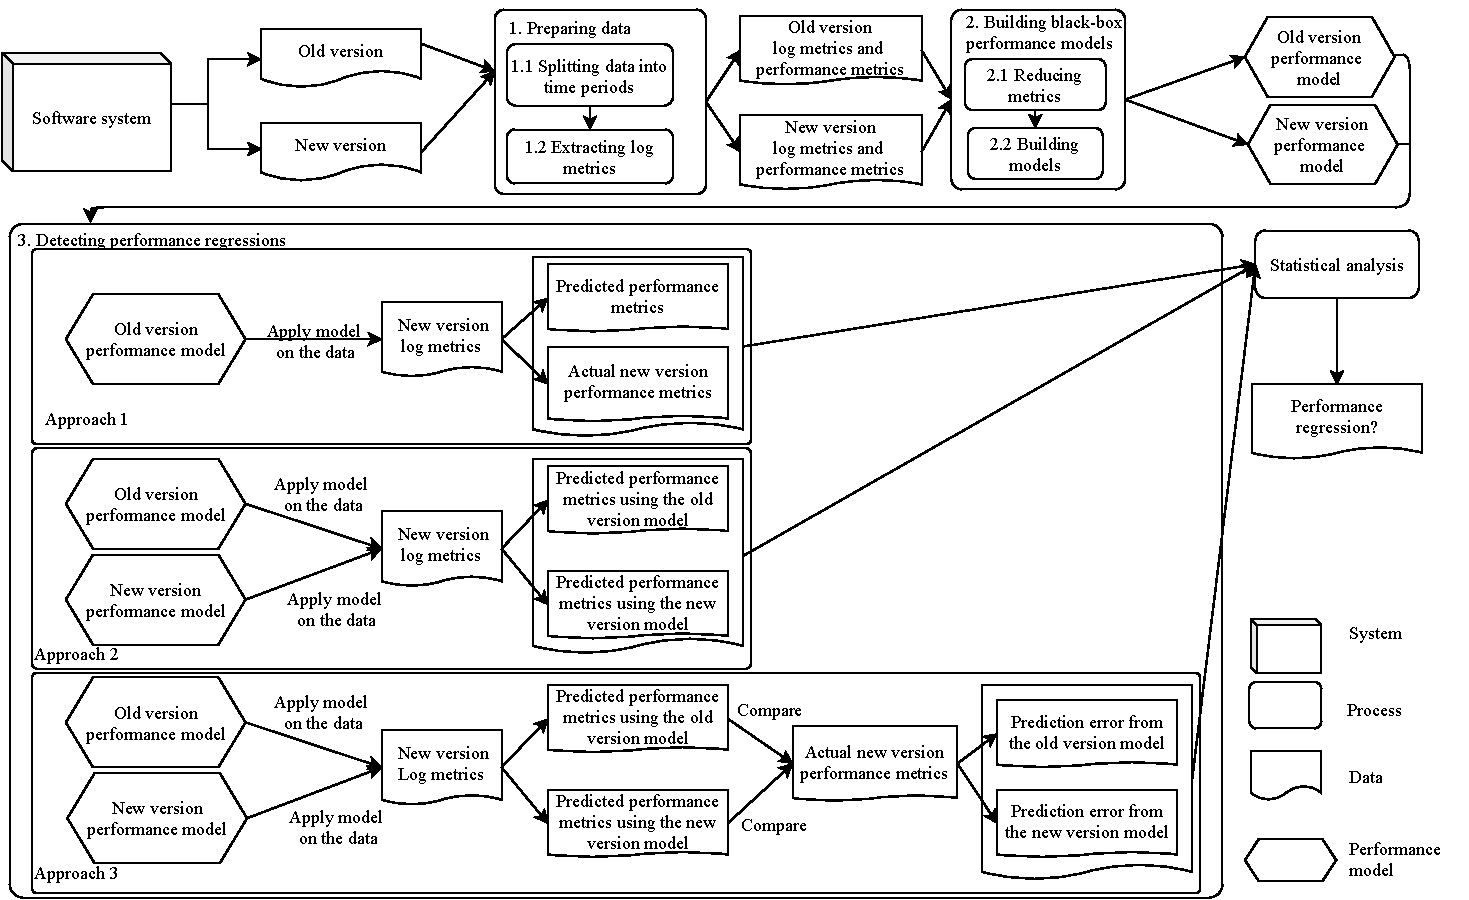
\includegraphics[width=\textwidth]{overview.pdf}
  \caption{An overview of our studied approaches of detecting performance regressions.}
  \label{fig:overview}
\end{figure*}

\subsection{Building black-box performance models}
\label{sec:buildmodel}
In this step, we build black-box models based on the log metrics and performance metrics that are collected and calculated from the data that is generated during system runtime under varied workloads. 

\subsubsection{Reducing metrics}
The frequency of some log events (e.g., periodical events) may not change over time.
The constant appearance of such events may not provide information about the changes in system workloads.
Therefore, after we calculate the log metrics of each log event, we reduce log metrics by removing redundant log metrics or log metrics with constant values in both previous and current versions. We first remove log metrics that have zero variance in both versions of the performance tests. 

Different log events may always appear at the same time, e.g., user logging in and checking user's privilege, and provide repetitive information for the workloads. To avoid bias from such repetitive information, we then perform correlation analysis and redundancy analysis on the log metrics. We calculate Pearson's correlation coefficient~\citep{benesty2009pearson} between each pair of log metrics. If a pair of log metrics have a correlation higher than $0.7$, we remove the one that has a higher average correlation with all other metrics. 
We repeat the process until there exists no correlation higher than $0.7$. The redundancy analysis would consider a log metric redundant if it can be predicted from a combination of other log metrics. We use each log metric as a dependent variable and use the rest of the log metrics as independent variables to build a regression model. We calculate the $R^2$ of each model. If the $R^2$ is larger than a threshold (e.g., 0.9), the current dependent variable (i.e., the log metric) is considered redundant. We then remove the log metric with the highest $R^2$ and repeat the process until no log metrics can be predicted with an $R^2$ higher than the threshold. 

We only apply this step when using traditional statistical models or machine learning models (like linear regression or random forest), while if a deep neural network (like convolutional neural network or recurrent neural network) is adopted to build the black-box performance models, we skip this step.


\subsubsection{Building models}
We build models that capture the relationship between a certain workload that is represented by the logs and the system performance. In particular, the independent variables are the log metrics from the last step and the dependent variable is the target performance metric (e.g., CPU usage). One may choose different types of statistical, machine learning or deep learning models, as our approach is agnostic to the choice of models. However, the results of using different types of models may vary (cf. RQ1). 


\subsection{Detecting performance regressions} \label{sec:comparions-approaches}

The goal of building performance models is to detect performance regressions. Therefore, in this step, we use the black-box performance models that are built from an old version of the system to predict the expected system performance of a new version. Then, we use statistical analysis to determine whether there exists performance deviance based on prediction errors of the models.

Intuitively, one may use the model that is built from the old version of the system to predict the performance metrics from running the new version of the system. By measuring the prediction error, one may be able to determine whether there exists performance deviance~\citep{DBLP:conf/osdi/CohenCGKS04,DBLP:conf/wosp/NguyenAJHNF12}. However, such a naive approach may be biased by the choice of thresholds that are used to determine whether there is performance deviance. For example, a well-built performance model may only have less than 5\% average prediction error; while another less fit performance model may have 15\% average prediction error. In these cases, it is challenging to determine whether an average prediction error of 10\% on the new version of the system should be considered as a performance regression. Therefore, statistical analyses are used to detect performance regressions in a systematic manner~\citep{DBLP:conf/icst/GaoJBL16,DBLP:conf/wosp/ShangHNF15,Foo:2015:ICS:2819009.2819034}. 

In particular, we leverage three approaches to detect performance regressions: \emph{Approach 1}) by comparing the predicted performance metrics (using the model built from the old version) and the actual performance metrics of the new version, \emph{Approach 2}) by comparing the predicted performance metrics of the new version using the model built from the old version and the model built from the new version, and \emph{Approach 3}) by comparing the prediction errors of the performance metrics on the new version using the model built from the old version and the model built from the new version. We describe each approach in detail in the rest of this subsection.

\noindent\textbf{Approach 1: }\emph{comparing the predicted performance metrics (using the model built form the old version) and the actual performance metrics of the new version.} %\hfill
The most intuitive way of detecting performance regression is to compare the predicted value and the actual value of performance metrics. Since the model is built from the old version of the system, if there exists a large error between the predicted value and the actual value of the performance metrics from the new version of the system, we may consider the existence of performance regressions. In particular, we use the data from the old version of the system, i.e., $Data_{old}$ to build a black-box performance model $Model_{old}$ (cf. Section~\ref{sec:buildmodel}). Afterward, we apply the model $Model_{old}$ on the data from the new version of the system, i.e., $Data_{new}$. Then we compare the predicted and the actual values of the performance metrics.


\noindent\textbf{Approach 2: }\emph{comparing the predicted performance metrics of the new version using the model built from the old version and the model built from the new version.} %\hfill
Since our approach aims to be applied to varying workloads, the performance regression may only impact a small number of time periods, while the source code with performance regressions may not be executed in other time periods. Therefore, only the time periods that are impacted by the performance regressions may contain large prediction errors. To address such an issue, we also built a performance model $Model_{new}$ using the data from the new version of the system ($Data_{new}$). 
This way, $Model_{new}$ is built using the data with potential performance regressions. 
Afterwards, we use $Model_{old}$ and $Model_{new}$ to predict the performance metrics in $Data_{new}$. 

Since $Model_{new}$ is built from $Data_{new}$, there exist a bias when applying $Model_{new}$ on $Data_{new}$. To avoid the bias, instead of building one $Model_{new}$, we build $n$ models, where $n$ is the number of data points that exist in $Data_{new}$. In particular, for each data point in $Data_{new}$, we build a performance model $Model_{new}^n$ by excluding that data point and apply the model $Model_{new}^n$ on the excluded data point. Therefore, for $n$ data points from $Data_{new}$, we end up having $n$ models and $n$ predicted values. 

Finally, we compare the predicted values using $Model_{old}$ on $Data_{new}$, and the predicted values by applying each $Model_{new}^n$ on each of the $n$ data points in $Data_{new}$.


\noindent\textbf{Approach 3: }\emph{comparing the prediction errors on the new version using the model built from the old version and the model built from the new version.}
The final approach of detecting performance regression is similar to the previous one (Approach 2), where instead of directly comparing the predicted performance metrics, we compare the distribution of the prediction errors by applying $Model_{old}$ on $Data_{new}$, and the predicted errors by applying each $Model_{new}^n$ on each of the $n$ data points in $Data_{new}$. The intuition is that when $Model_{old}$ has a larger prediction error than $Model_{new}$, it may be an indication of performance deviance between the two versions. We note that this approach would only be able to determine whether there exists performance deviance, which may actually be improvement instead of regression. 


\noindent\textbf{Statistical analysis.}
All three approaches generate two distributions of either actual/predicted performance metric values, or prediction errors. With two distributions of data at hand, we compare the two distributions similar to previous studies~\citep{Chen:2016:CHD:2950290.2950303} using statistical tests and effect sizes. In particular, we use the Mann-Whitney U test since it is non-parametric and it does not assume a normal distribution of the compared data. we run the test at the 5\% level of significance, i.e., if the P-value of the test is not greater than 0.05, we would reject the \emph{null hypothesis} in favor of the alternative hypothesis, i.e., there exists a statistically significant difference between the two distributions. In order to study the magnitude of the difference without being biased by the size of the data, we further adopt the effect size as a complement
of the statistical significance test. Considering the non-normality of our data points, we
utilize \emph{Cliff's Delta}~\citep{cliff1996ordinal} using the
thresholds provided in prior research~\citep{romano2006appropriate}.




\section{Case Study Setup} \label{sec:casestudysetup}
To study the effectiveness of our approaches for detecting performance regressions under varying workloads, we perform case studies on two open source systems and one large-scale industrial system\footnote{Our experimental setup, workloads and results are shared online \url{https://github.com/senseconcordia/ICPE2020Data} as a replication package.}. In this section, we first present the subject systems. Then, we present the workloads applied to the systems, the experimental environment and performance issues. Finally, we present the choices of machine learning models that are used in our approaches. 

\subsection{Subject systems}
We evaluate our approaches with two open-source systems, namely OpenMRS and Apache James, as well as one industrial system (System X). Apache James is a Java-based mail server. OpenMRS is an open-source health care system that support customized medical records and it is wildly used in developing countries. System X is a commercial software that provides government-regulation related reporting services. The service is wildly used as the market leader of the domain. Due to a Non-Disclosure Agreement (NDA), we cannot reveal additional details about the system. We do note that System X has over ten years of history with more than two million lines of code that are based on Microsoft .Net. All our subject systems cover different domains and are studied in prior research~\citep{Yao:2018:LSL:3184407.3184416, DBLP:conf/icst/GaoJBL16}. The details of each subject system are shown in Table~\ref{tab:subjects}. 


% Table generated by Excel2LaTeX from sheet 'Sheet4'
\begin{table}[tbh]
  \centering
%   \vspace{-0.3cm}
%   \small
  \caption{Overview of our subject systems}
%   \vspace{-0.2cm}
    \begin{tabular}{c|c|c|r}
    \hline
    Subjects & Versions & Domains & SLOC (K) \\
    \hline
    OpenMRS & 2.1.4 & Medical & 67 \\
    
    Apache James & 2.3.2, 3.0M1, 3.0M2 & Mail Server & 37 \\
    
    System X & 10 releases in 2019 & Commercial & \textgreater 2,000 \\
    \hline
    \end{tabular}%
  \label{tab:subjects}%
%   \vspace{-0.5cm}
\end{table}%


\subsection{Subject workload design}
\subsubsection{OpenMRS}
OpemMRS provides a web-based interface and RESTFul services. We used the default OpenMRS demo database in our performance tests. The demo database contains data for over 5K patients and 476K observations. OpenMRS contains four typical scenarios: adding, deleting, searching and editing operations. We designed five different performance tests that are composed of eight various test actions, e.g., searches of patients, concepts, encounters, and observations, and creation, deletion and edit of patient information. Those five performance tests are distinguished by the ratio of each action. In order to simulate a more realistic workload in the field, we added random controllers and random order controllers in JMeter to vary the workload. Moreover, we also simulated the variety of the amount of users and activities in the field by setting random gaps between the repetitions of each user’s activities, randomizing the order of the user activities and for different workloads and different time, setting different number of maximum concurrent users. The original version, i.e., v0 of OpenMRS does not have any injected or known performance regressions. We separately injected four performance regressions (heavier DB request, additional I/O, constant delay and additional calculation) into v0. These four versions are called v1, v2, v3, and v4, respectively. The details of the injected performance regressions of OpenMRS are shown in Table~\ref{tab:workloaddeisign}.

We deployed the OpenMRS on two machines, each with Intel Core i5-2400 CPU (3.10GHz), 8 GB memory, 512GB SATA hard drive. One machine is deployed as application server and another machine is deployed as MySQL database server. We used the RESTFul API from OpenMRS and ran JMeter on five extra machines with the same specification to simulate users in the client side with a five-hours workload. Each machine hosts one JMeter instance with one type of workload. We used \emph{Pidstat}~\citep{pidstat} to monitor CPU usage as the performance metrics of this study.
To minimize the noise from the system warm-up and cool-down periods, we filtered out the data from the first and last half an hour of running each workload. Thus, we only kept four hours of data from each performance test.
%\vspace{-0.25cm}
\subsubsection{Apache James}
Apache James is an open source enterprise mail server. It contains two main scenarios: sending and retrieving mails. Those two actions can be further divided into many smaller scenarios, e.g., sending mails with or without attachments and retrieving entire mail or only the header of the mail. In total, we built eight scenarios for the performance test. Similar to OpenMRS, we also created five different workloads that consist of eight actions of different ratio and performance-test Apache James with varying workloads to simulate the real user operation. We used JMeter to create performance tests that exercise Apache James. Different from OpenMRS, in which the performance regressions are manually injected, we performance-tested on three different versions of systems with known real-world performance issues for Apache James. Apart from the last stable version 2.3.2, there are multiple Milestone Releases for version 3.0. After checking the release notes on the Apache James website, we picked 3.0M1 and 3.0M2 to use in our study. These three selected versions have many bug fixes and performance improvements~\citep{Apache-James}. The same subjects are studied in a prior research on performance testing~\citep{DBLP:conf/icst/GaoJBL16}. Table~\ref{tab:workloaddeisign} summarizes the details of performance improvements of three selected versions. 

We deployed Apache James on a server machine with an Intel Core i7-8700K CPU (3.70GHz), 16 GB memory on a 3TB SATA hard drive. We ran JMeter on five extra machines with Intel Core i5-2400 CPU (3.10GHz), 8 GB memory and 320GB SATA hard drive to generate multiple five-hour workloads. Similar to OpenMRS, we use \emph{Pidstat}~\citep{pidstat} to monitor CPU usage as the performance metrics of this study. We filtered out the data form the first and last half an hour of running each workload to minimize the system noises. 

\subsubsection{System X}
System X is deployed in production and is used by real users worldwide. We retrieved the execution logs and the corresponding CPU usage on a daily basis. The System X is deployed in an internal production environment. Due to the NDA, we cannot reveal additional details about the hardware environment and the usage scenarios of System X.

% \begin{table}
% \caption{Performance regressions in the subject systems}
% \tabcolsep=0.1cm
% \small
% \label{tab:workloaddeisign}
% \begin{tabular}{ccccl}
%  \toprule
% System & \begin{tabular}[c]{@{}l@{}}\# of Test \\ Actions\end{tabular} & Versions & \begin{tabular}[c]{@{}l@{}}\# of Test\\ Workloads\end{tabular} & Performance Issues \\
% \midrule
%  &  & v0 & 4 \& 5 & Original version \\
%  &  & v1 & 4 \& 5 & Injected Busy loop \\
% OpenMRS & 8 & v2 & 4 \& 5 & Added additional IO \\
%  &  & v3 & 4 \& 5 & Created a constant delay \\
%  &  & v4 & 4 \& 5 & \begin{tabular}[c]{@{}l@{}}Add additional \\ calculations\end{tabular} \\
%  \midrule
%  &  & 2.3.2 & 4 \& 5 & Stable release version \\
% Apache James & 8 & 3.0M1 & 4 \& 5 & \begin{tabular}[c]{@{}l@{}}Improved ActiveMQ \\ spool efficiency\end{tabular} \\
%  &  & 3.0M2 & 4 \& 5 & \begin{tabular}[c]{@{}l@{}}Improved large attachment\\ handling efficiency\end{tabular} \\
%  \bottomrule
% \end{tabular}
% \end{table}

% Table generated by Excel2LaTeX from sheet 'Sheet4'

\begin{table}[tbh]
  \centering
%   \vspace{-0.3cm}
%   \footnotesize
  \caption{Performance regressions in the studied open source systems}
%   \vspace{-0.2cm}
    \begin{tabular}{c|c|p{3.3cm}}
    \hline
    System & Versions & \multicolumn{1}{c}{Performance regressions} \\
    \hline
          & v0    & \multicolumn{1}{c}{Original version} \\
\cline{2-3}          & v1    & \multicolumn{1}{c}{Injected heavier DB request} \\
\cline{2-3}    OpenMRS & v2    & \multicolumn{1}{c}{Added additional I/O access} \\
\cline{2-3}          & v3    & \multicolumn{1}{c}{Created a constant delay} \\
\cline{2-3}          & v4    & \multicolumn{1}{c}{Injected additional calculation} \\
    \hline
          & 2.3.2 & \multicolumn{1}{c}{Stable release version} \\
          \cline{2-3}
          Apache James & 3.0M1 & \multicolumn{1}{c}{Improved ActiveMQ spool efficiency~\citep{Apache-James}} \\
          \cline{2-3}
          & 3.0M2& \multicolumn{1}{c}{Improved large attachment handling efficiency~\citep{Apache-James}} \\
    \hline
    \end{tabular}%
  \label{tab:workloaddeisign}%
%   \vspace{-0.5cm}
\end{table}%



\subsection{Subject models}
Our approach presented in Section~\ref{sec:approach} is not designed strictly to any particular type of machine learning models. In fact, practitioners may choose their preferred models. In this study, we study the use of six different types of models, namely linear regression, random forest, XGBoost, convolutional neural network (CNN), recurrent neural network (RNN) and long short-term memory (LSTM). In particular, for linear regression, random forest, XGBoost and CNN, the input of the models are vectors whose values are the number of appearance of each log event in a time period. For RNN and LSTM, we sort the logs in each time period by their corresponding time stamp to create a sequence as the input of the neural networks. Our XGBoost model is fine-tuned using the GridSearchCV~\citep{girdsearcv} method. Our CNN, RNN and LSTM have three, four and four layers, respectively, and they are trained with five, five and ten epochs, respectively. The number of layers and epochs are manually fine-tuned to avoid overfitting.
 


\section{Case Study Results} \label{sec:casestudyresults}
In this section, we evaluate our approaches by answering two research questions.

\subsection*{RQ1: How well can we model system performance under varying workloads?}

\subsubsection*{Motivation}
In order to use black-box machine learning models to detect performance regressions under varying workloads, we first need to understand whether such black-box models could accurately model the performance of a software system under varying workloads.
Although prior research demonstrates promising results of using black-box models to capture the relationship between system performance and logs~\citep{Yao:2018:LSL:3184407.3184416,DBLP:conf/issre/FarshchiSWG15},
these models are built on predefined in-house workloads instead of varying field workloads. 
If such black-box models are sensitive to the variance in the workloads, they may not be suitable for modeling the performance of software systems under the field workloads from real end users.

\subsubsection*{Approach}
In order to understand the black-box models' ability for modeling system performance under varying workloads, we train the models on one set of workloads and evaluate the performance of the models on a different set of workloads (i.e., \emph{unseen} workloads).

\noindent\textbf{Modeling for the open source systems. }
For each open source system (i.e., OpenMRS and Apache James), we select the version of the system that is without performance regressions. We first run the system with four different concurrent workloads (i.e., \emph{4W}) and collect the logs and performance metrics. In order to ensure having new workloads to the system, we conduct another run by having an additional concurrent workload, i.e., having five different concurrent workloads (i.e., \emph{5W}). We build the performance models using the data that is generated by running the \emph{4W} workloads (\emph{a.k.a.} the training set) and apply the model on the data that is generated by running the \emph{5W} workloads (\emph{a.k.a.} the testing set). 
The training and testing sets are derived from independent system runs. 
We evaluate the prediction performance of the black-box models on the 5W workloads by comparing the predicted performance and the measured performance.

\noindent\textbf{Modeling for the industrial system. }
For System X, we directly use the field data that is generated by workloads from the real end users. For each release cycle with $n$ days, we use the data from the first $n/2$ days to build the models and apply them on the data from the second $n/2$ days to evaluate the prediction performance of the models. We would like to note that there exists no control on the end users for applying any particular workload, and that all the data is directly retrieved from the field with no interference on the behavior of the end users. 

\noindent\textbf{Analysis of modeling results. }
We calculate the prediction errors of the models on the new workloads (i.e., the \emph{5W} workloads for the open source systems and the second $n/2$-day workloads for System X).
In order to understand the magnitude of the prediction errors, we use the prediction errors of the models on the old workloads (i.e., the $4W$ workloads for the open source systems and the first $n/2$-day workloads for System X) as baselines. The baseline prediction errors are calculated using a 10-fold cross validation to avoid the bias of having the same training and testing data.  
\begin{itemize}
    \item \textbf{Median relative error}. The difference between the predicted performance and the measured performance, normalized by the measured performance.
    \item \textbf{p-value} (Mann-Whitney U). In order to understand whether the models trained on the old workloads can equivalently capture the system performance under the new workloads, we use the Mann-Whitney U test~\citep{nachar2008mann} to determine whether there exists a statistically significant difference (i.e., p-value $<$ 0.05) between the prediction errors on the new workloads and the prediction errors on the old workloads. 
    \item \textbf{Effect size} (Cliff\textquotesingle s delta). Reporting only the statistical significance may lead to erroneous results (i.e., if the sample size is very large, the p-value can be very small even if the difference is trivial)~\citep{sullivan2012using}. Therefore, we apply Cliff\textquotesingle s Delta~\citep{cliff1996ordinal} to quantify the effect size of the difference between the prediction errors on the old workloads and the prediction errors on the new workloads. 
\end{itemize}

\subsubsection*{Results}
Table \ref{tab:model_error} shows the detailed results of using six machine learning techniques to model the performance of the studied open source systems (i.e., OpenMRS and Apache James) under varying workloads.
 The column ``MRE'' shows the median relative errors of applying the models (trained on the \emph{4W} workloads) on the \emph{4W} workloads and the \emph{5W} workloads, respectively. 
  The columns ``p-value'' and ``effect size'' show the statistical significance and the effect size of the difference between the prediction errors of the models on the \emph{4W} workloads and the prediction errors of the models on the \emph{5W} workloads, respectively. The ``violin plot'' column shows the distribution of the relative prediction errors under the \emph{4W} and \emph{5W} workloads.

\begin{landscape}

\begin{table*}[htbp]
  \centering
  \footnotesize
  \caption{Prediction error details for OpenMRS and Apache James under different workloads. 
 }
    
    \resizebox{.66\paperheight}{!}{
    \begin{tabular}{|c|c|c|c|c|c|c|c|c|c|c|}
    \hline
    \multirow{2}[4]{*}{Model} & \multicolumn{5}{c|}{OpenMRS}          & \multicolumn{5}{c|}{Apache James} \\
\cline{2-11}          & \multicolumn{2}{c|}{MRE} & P-value & Effect size & Violin plot & \multicolumn{2}{c|}{MRE} & P-value & Effect size & Violin plot \\
    \hline
    \multicolumn{1}{|c|}{\multirow{2}[9]{*}{Linear 
Regression}} & \multirow{1}[5]{*}{4W}    & \multirow{1}[5]{*}{3.12\%} & \multirow{2}[9]{*}{\textless 0.01} & \multirow{1}[10]{*}{-0.08} & \multirow{2}[4]{*}{ {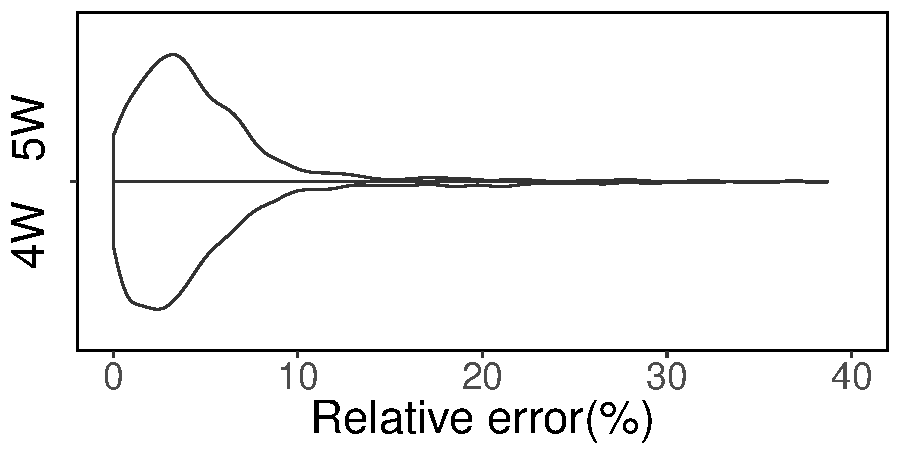
\includegraphics[height=15mm,width=30mm]{openmrs_linear_regression.pdf}}} & \multirow{1}[5]{*}{4W}    & \multirow{1}[5]{*}{23.24\%} & \multirow{2}[9]{*}{0.41} & \multicolumn{1}{c|}{\multirow{2}[9]{*}{N/A}} & \multirow{2}[4]{*}{{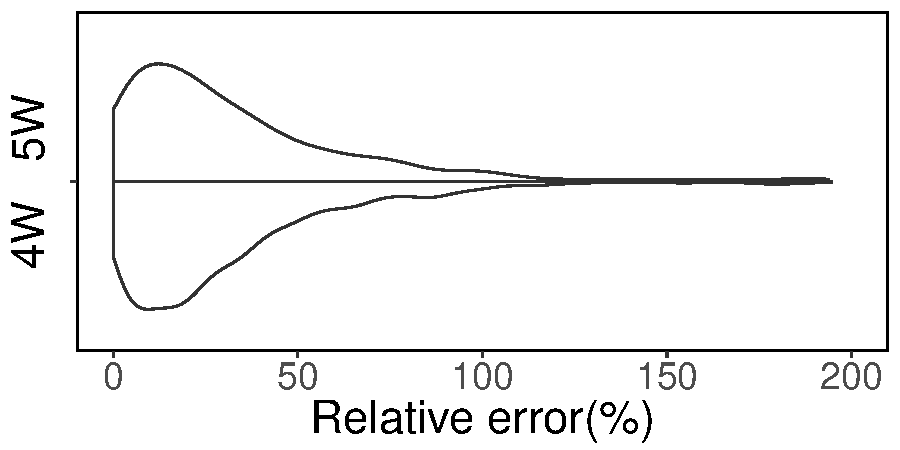
\includegraphics[height=15mm,width=30mm]{jms_linear_regression.pdf}}} \\[4.5mm]
\cline{2-3}\cline{7-8}          & \multirow{1}[5]{*}{5W}    & \multirow{1}[5]{*}{3.58\%} &       & (negligible) &       & \multirow{1}[5]{*}{5W}    & \multirow{1}[5]{*}{23.76\%} &       &       &  \\[4.5mm]
    \hline
    \multicolumn{1}{|c|}{\multirow{2}[9]{*}{Random 
Forest}} & \multirow{1}[5]{*}{4W}    & \multirow{1}[5]{*}{2.36\%} & \multirow{2}[9]{*}{\textless 0.01} & \multirow{1}[10]{*}{-0.09} & \multirow{2}[4]{*}{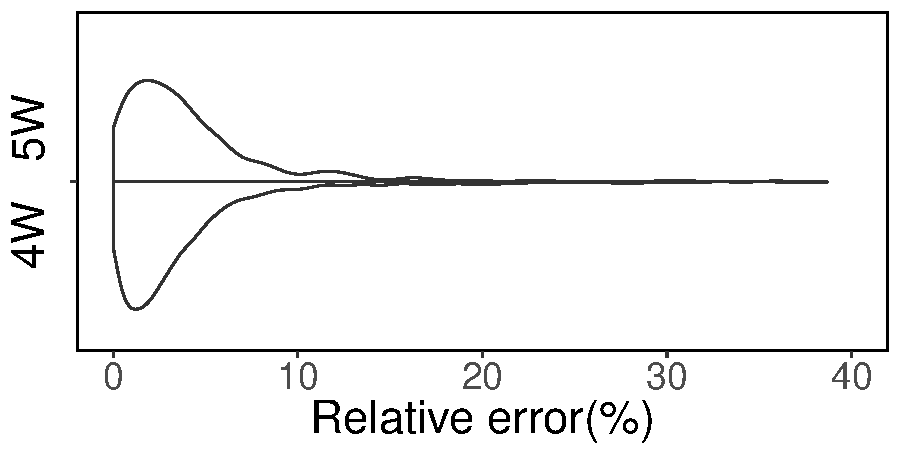
\includegraphics[height=15mm,width=30mm]{openmrs_random_forest.pdf}} & \multirow{1}[5]{*}{4W}    & \multirow{1}[5]{*}{22.99\%} & \multirow{2}[9]{*}{0.42} & \multicolumn{1}{c|}{\multirow{2}[9]{*}{N/A}} & \multirow{2}[4]{*}{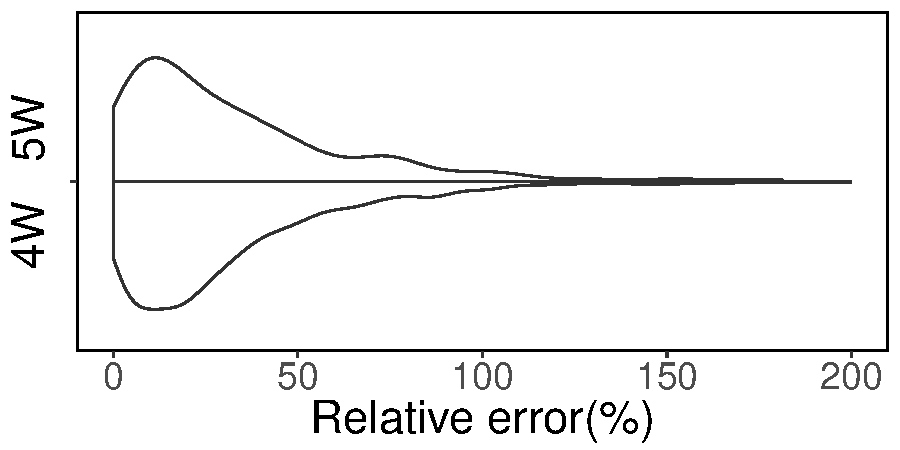
\includegraphics[height=15mm,width=30mm]{jms_random_forest.pdf}} \\[4.5mm]
\cline{2-3}\cline{7-8}          & \multirow{1}[5]{*}{5W}    & \multirow{1}[5]{*}{2.90\%} &       & (negligible) &       & \multirow{1}[5]{*}{5W}    & \multirow{1}[5]{*}{23.08\%} &       &       &  \\[4.5mm]
    \hline
    \multirow{2}[9]{*}{XGBoost} & \multirow{1}[5]{*}{4W}    & \multirow{1}[5]{*}{2.16\%} & \multirow{2}[9]{*}{0.14} & \multirow{2}[9]{*}{N/A} & \multirow{2}[4]{*}{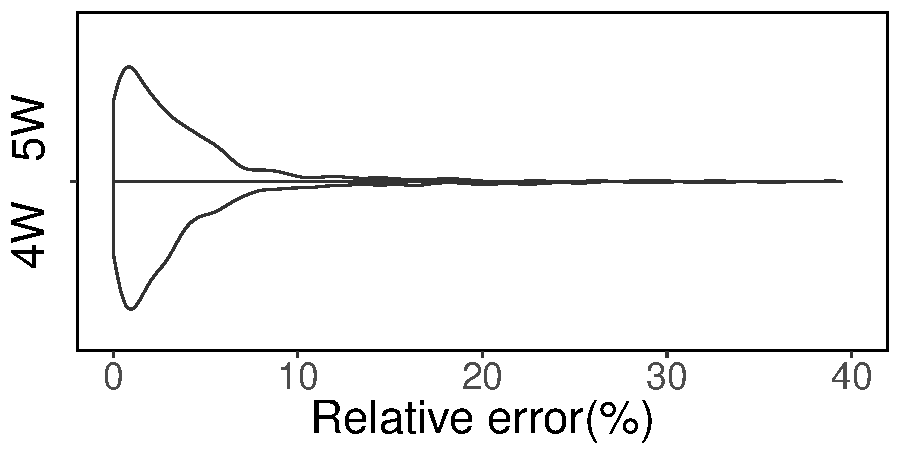
\includegraphics[height=15mm,width=30mm]{openmrs_xgboost.pdf}} & \multirow{1}[5]{*}{4W}    & \multirow{1}[5]{*}{24.29\%} & \multirow{2}[9]{*}{0.44} & \multirow{2}[9]{*}{N/A} & \multirow{2}[4]{*}{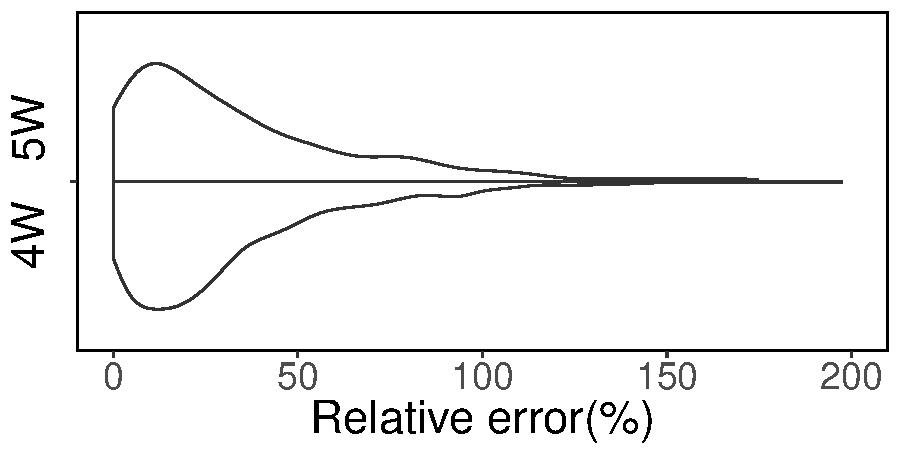
\includegraphics[height=15mm,width=30mm]{jms_xgboost.pdf}} \\[4.5mm]
\cline{2-3}\cline{7-8}          & \multirow{1}[5]{*}{5W}    & \multirow{1}[5]{*}{2.11\%} &       &       &       & \multirow{1}[5]{*}{5W}    & \multirow{1}[5]{*}{24.42\%} &       &       &  \\[4.5mm]
    \hline
    \multirow{2}[9]{*}{CNN} & \multirow{1}[5]{*}{4W}    & \multirow{1}[5]{*}{9.56\%} & \multirow{2}[9]{*}{\textless 0.01} & \multirow{1}[10]{*}{0.12} & \multirow{2}[4]{*}{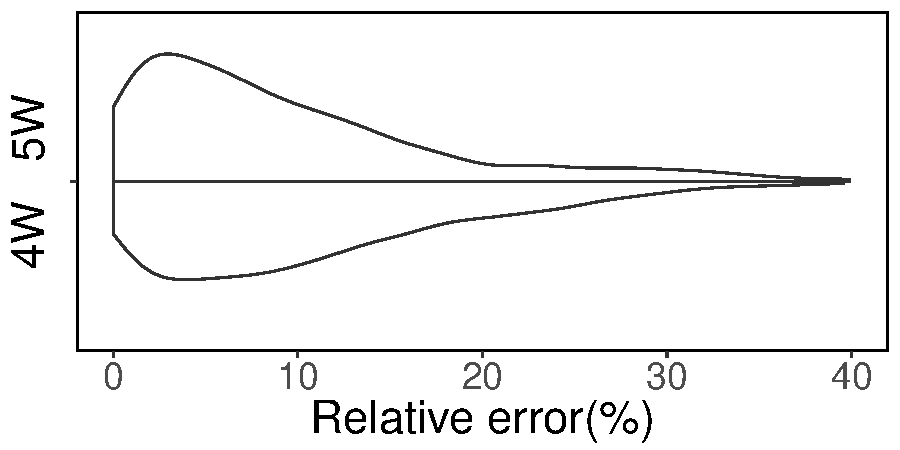
\includegraphics[height=15mm,width=30mm]{openmrs_cnn.pdf}} & \multirow{1}[5]{*}{4W}    & \multirow{1}[5]{*}{33.61\%} & \multirow{2}[9]{*}{0.11} & \multicolumn{1}{c|}{\multirow{2}[9]{*}{N/A}} & \multirow{2}[4]{*}{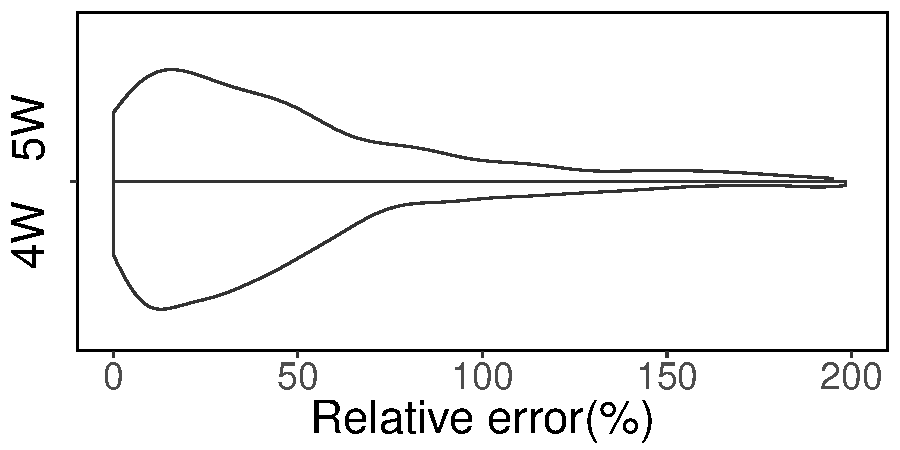
\includegraphics[height=15mm,width=30mm]{jms_cnn.pdf}} \\[4.5mm]
\cline{2-3}\cline{7-8}          & \multirow{1}[5]{*}{5W}    & \multirow{1}[5]{*}{7.47\%} &       & (negligible) &       & \multirow{1}[5]{*}{5W}    & \multirow{1}[5]{*}{37.51\%} &       &       &  \\[4.5mm]
    \hline
    \multirow{2}[9]{*}{RNN} & \multirow{1}[5]{*}{4W}    & \multirow{1}[5]{*}{5.63\%} & \multirow{2}[9]{*}{0.32} & \multirow{2}[9]{*}{N/A} & \multirow{2}[4]{*}{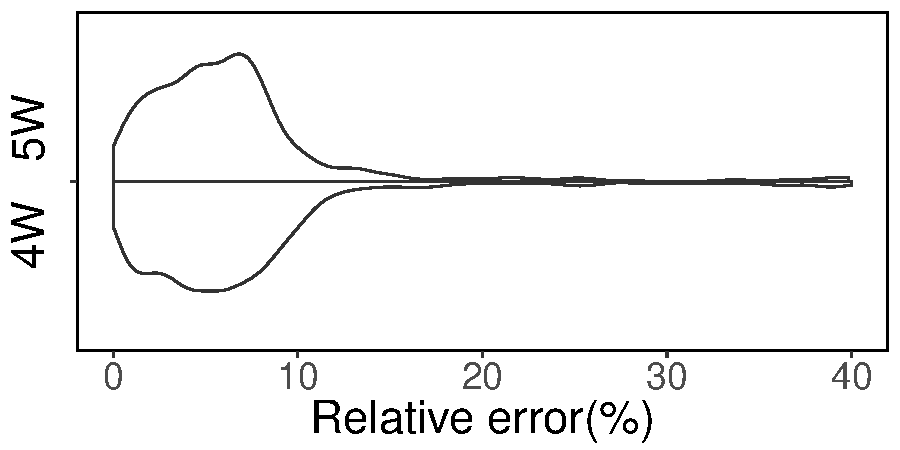
\includegraphics[height=15mm,width=30mm]{openmrs_rnn.pdf}} & \multirow{1}[5]{*}{4W}    & \multirow{1}[5]{*}{51.34\%} & \multirow{2}[9]{*}{0.01} & \multirow{1}[10]{*}{0.07} & \multirow{2}[4]{*}{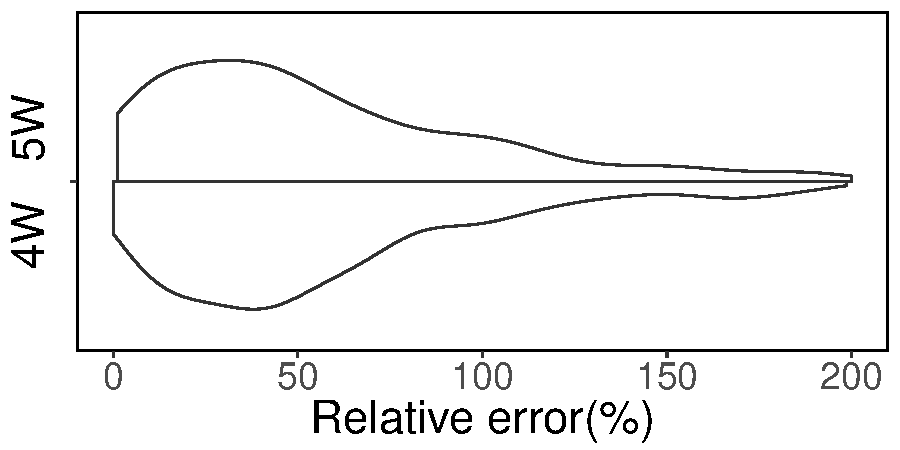
\includegraphics[height=15mm,width=30mm]{jms_rnn.pdf}} \\[4.5mm]
\cline{2-3}\cline{7-8}          & \multirow{1}[5]{*}{5W}    & \multirow{1}[5]{*}{5.73\%} &       &       &       & \multirow{1}[5]{*}{5W}    & \multirow{1}[5]{*}{47.22\%} &       & (negligible) &  \\[4.5mm]
    \hline
    \multirow{2}[9]{*}{LSTM} & \multirow{1}[5]{*}{4W}    &\multirow{1}[5]{*}{ 4.53\%} & \multirow{2}[9]{*}{\textless 0.01} & \multirow{1}[10]{*}{-0.25} & \multirow{2}[4]{*}{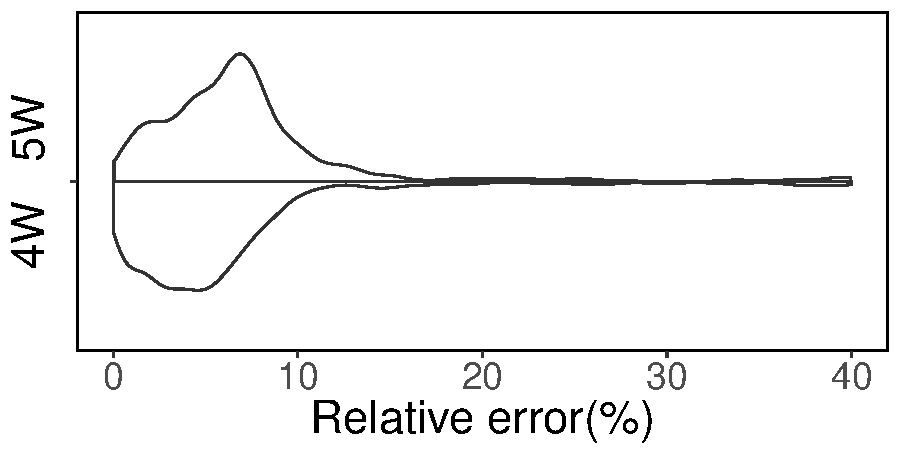
\includegraphics[height=15mm,width=30mm]{openmrs_lstm.pdf}} & \multirow{1}[5]{*}{4W}    & \multirow{1}[5]{*}{34.88\%} & \multirow{2}[9]{*}{\textless 0.01} & \multirow{1}[10]{*}{-0.27} & \multirow{2}[4]{*}{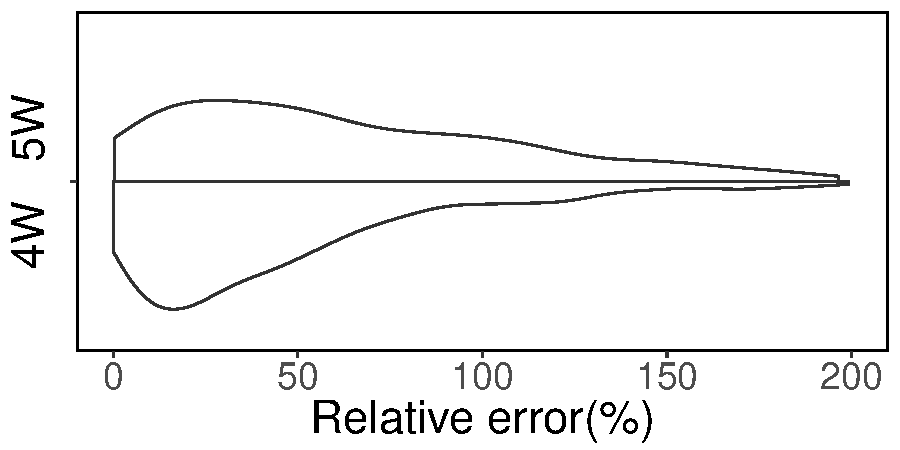
\includegraphics[height=15mm,width=30mm]{jms_lstm.pdf}} \\[4.5mm]
\cline{2-3}\cline{7-8}          & \multirow{1}[5]{*}{5W}    & \multirow{1}[5]{*}{6.42\%} &       & (small) &       & \multirow{1}[5]{*}{5W}    & \multirow{1}[5]{*}{57.11\%} &       & (small) &  \\[4.5mm]
    \hline
    \end{tabular}}
    Note: The column ``MRE'' presents the median relative errors.\hfill
  \label{tab:model_error}%
\end{table*}%
\end{landscape}

\noindent\textbf{Our black-box models can effectively model the performance of the studied systems using the dynamic runtime activities that are recorded in the logs.} 
As shown in Table \ref{tab:model_error}, the XGBoost model achieves the best results for modeling the performance of the OpenMRS system, with a median relative error of 2.11\% on the \emph{5W} workloads (i.e., the new workloads) and a median relative error of 2.16\% on the \emph{4W} workloads (i.e., the baseline workload). 
The random forest model achieves the best results for Apache James, reaching a median relative error of 22.99\% and 23.08\% for the \emph{4W} workloads and \emph{5W} workloads, respectively. 
All the machine learning models achieve better results for the OpenMRS system than the results for the Apache James system.
The less-promising results for the Apache James system might be explained by the latency between the actual activities of the mail server system and the recorded logs. For example, the system can take an extended period of time to process an email with a large attachment, while a log about the successful processing of the email is only printed after the processing period.

\noindent\textbf{The traditional models (e.g., linear regression and random forest) outperform the deep neural networks (e.g., CNN and RNN) for modeling the performance of the studied systems.}
As shown in Table~\ref{tab:model_error}, for both the OpenMRS and the Apache James systems, the three traditional models achieve better results than the three deep neural networks for modeling the system performance.
These results indicate that the relationship between the system performance and the runtime activities recorded in the logs can be effectively captured by the simple traditional models.
Such results also agree with a recent study~\citep{DacremaArxiv2019} that compares deep neural networks and traditional models for the application of automated recommendations.


\noindent\textbf{Our black-box models can equivalently explain the performance of a system under new workloads that are unseen when constructing the models.}
Table~\ref{tab:model_error} shows the statistical significance (i.e. the p-value) and the effect size of the difference between the prediction errors of applying the old models (i.e., trained from the \emph{4W} workloads) on the new workloads (i.e., the \emph{5W} workloads) and applying the old models on the old workloads (i.e., the \emph{4W} workloads). 
Table \ref{tab:model_error} also compares the distributions of the prediction errors for the \emph{4W} and \emph{5W} workloads.
The prediction errors of most of the models (except LSTM) have an either statistically insignificant or negligible difference between the \emph{4W} and the \emph{5W} workloads, indicating that the models trained from the old workloads can equivalently model the system performance under new workloads.
The LSTM model results in a \emph{small} difference of the prediction errors between the \emph{4W} and the \emph{5W} workloads. We suspect that the complex LSTM model is likely to over-fit towards the training workloads.

Due to an NDA, the detailed results of using the machine learning techniques to model the performance of the industry system (i.e., System X) are not presented in this paper. However, the results are similar to the shown results for the open source systems. In particular, when modeling the performance of all 10 studied versions of System X, the prediction errors are all between 10\% to 20\%. In addition, when we evaluate the models with different workloads, the differences between prediction errors are all either statistically insignificant or with negligible/small effect sizes.



\hypobox{Simple traditional models (e.g., linear regression and random forest) can effectively capture the relationship between the performance of a system and its dynamic activities that are recorded in logs, with varying workloads.
}

\subsection*{RQ2: Can our approach detect performance regressions under varying workloads?}

\subsubsection*{Motivation}

In traditional performance testing, in order to detect performance regressions, performance analysts compare the performance data of two versions of a software system that is generated by running the same workloads from the same performance test suites. 
However, in a field environment, as the workloads of the systems are constantly changing, it is almost impossible to run two software versions on the same workloads to detect performance regressions.
The results of RQ1 show that our black-box models can accurately capture the performance of a software system even under new workloads that are unseen when training the models.
Therefore, in this research question, we would like to leverage such black-box models to detect performance regressions when the workloads of the two versions of a system are not consistent.

Running the systems for hours or days before discovering performance regressions incurs a high cost. As the systems are already running in the field, any delay in detecting the performance regressions may pose a huge impact on the end users. Hence, the desired approach in practice should be able to detect performance regression in a timely manner. Therefore, we also want to study how fast our approaches can detect performance regressions. 

\subsubsection*{Approach}

The results from RQ1 show that random forest and XGBoost have the lowest prediction errors when modeling performance (cf. Table~\ref{tab:model_error}). Since XGBoost requires resource-heavy fine-tuning, we opt to use random forest in this research question. For the open source systems, we first build the performance models from running the systems without performance regressions under the \emph{4W} workloads (i.e., a combination of four different concurrent workloads). We then run the systems without performance regressions under the \emph{5W} workloads (i.e., a combination of five different concurrent workloads). Ideally, our approach should not detect performance regressions from these runs. 
We use such results as a baseline to evaluate the effectiveness of our approach for detecting performance regressions under the new workloads (i.e., the \emph{5W} workloads). 
Afterward, we run the systems with the performance regressions (cf. Table~\ref{tab:workloaddeisign}) under the \emph{5W} workloads. Our approach should be able to detect performance regressions from these runs.

For System X from the industry, for every new release, we use our approach to compare the field data from the new release and the previous release to determine whether there are performance regressions. Since there are no injected or pre-known performance regressions, we present the detected performance deviance to the developers of the systems and manually study the code changes to understand whether the detection results are correct. For the releases that are detected as not having performance regressions, we cannot guarantee that these releases are free of performance regressions. However, we also present the results to the developers to confirm whether there exist any users who report performance-related issues for these releases. If so, our detection results may be considered false.

Finally, to study how fast our approaches can detect performance regressions, for the new versions of the systems that have performance regressions, we only use the first 15-minute data and apply our approach to detect the performance regressions. Then, we follow an iterative approach to add another 5-minute data to the existing data, until our approach can detect the performance regressions (i.e., with a medium or large effect size that is higher than the baseline). 

\subsubsection*{Results}

\noindent\textbf{Our black-box-based approaches can effectively detect performance regressions under varying workloads.}
Table~\ref{tab:predictionresult_rq2} shows the results of our three approaches of performance regression detection (cf. Section~\ref{sec:comparions-approaches}) on OpenMRS and Apache James. We find that with all three approaches, when there are known performance regressions between two versions, the statistical analysis always shows a significant difference between the two versions with medium or large effect sizes. In addition, the effects sizes from Approach 1 and 2 are negative, confirming the existence of performance regressions (negative values indicate performance regression and positive values indicate performance improvement). 

When we compare the effect sizes with the baseline, i.e., running our approaches with systems without performance regressions but under two different workloads, we find that the baseline effect sizes are always smaller than the corresponding ones with performance regressions, except when detecting the regression in v3 of OpenMRS. We consider the reason being the nature of the regression in v3, i.e., an injected delay. Since our considered performance metric is the CPU usage and such a delay may not have a large impact on the CPU usage, it is difficult for our approaches to detect such a regression. 


\begin{table}[tbh]
  \centering
  \tiny
  \tabcolsep=0.14cm
  \caption{Performance regression detection results for OpenMRS and Apache James. }
    \begin{tabular}{|c|c|c|c|c|c|c|c|}
    \hline
    \multicolumn{8}{|c|}{OpenMRS} \\
    \hline
    \multicolumn{2}{|c|}{Versions} & \multicolumn{2}{c|}{Approach 1} & \multicolumn{2}{c|}{Approach 2} & \multicolumn{2}{c|}{Approach 3} \\
    \hline
    \multicolumn{1}{|p{0.7cm}<{\centering}|}{Old\newline{}version} & \multicolumn{1}{|p{0.7cm}<{\centering}|}{New\newline{}version} & \multirow{1}[3]{*}{P-value} & \multirow{1}[3]{*}{Effect size} & \multirow{1}[3]{*}{P-value} & \multirow{1}[3]{*}{Effect size} & \multirow{1}[3]{*}{P-value} & \multirow{1}[3]{*}{Effect size} \\
    \hline
    v0 & v0 & $\ll$0.001 & 0.39 (medium) &  $\ll$0.001 & 0.36 (medium) & $\ll$0.001 & 0.17(small) \\
    \hline
    v0 & v1 & $\ll$0.001 & -0.59 (large) & $\ll$0.001 & -0.69 (large) & $\ll$0.001 & 0.38 (medium) \\
    \hline
    v0 & v2 & $\ll$0.001 & -0.44 (medium) & $\ll$0.001 & -0.63 (large) & $\ll$0.001 & 0.37 (medium) \\
    \hline
    v0 & v3 & $\ll$0.001 & -0.36 (medium) & $\ll$0.001 & -0.42 (medium) & $\ll$0.001 & 0.53 (large) \\
    \hline
    v0 & v4 & $\ll$0.001 & -0.69 (large) & $\ll$0.001 & -0.76 (large) & $\ll$0.001 & 0.51 (large) \\
    \hline
    \hline
    \multicolumn{8}{|c|}{Apache James} \\
    \hline
    \multicolumn{2}{|c|}{Versions} & \multicolumn{2}{c|}{Approach 1} & \multicolumn{2}{c|}{Approach 2} & \multicolumn{2}{c|}{Approach 3} \\
    \hline
    \multicolumn{1}{|p{0.7cm}<{\centering}|}{Old \newline{}version} & \multicolumn{1}{|p{0.7cm}<{\centering}|}{New \newline{}version} & \multirow{1}[3]{*}{P-value} & \multirow{1}[3]{*}{Effect size} & \multirow{1}[3]{*}{P-value} & \multirow{1}[3]{*}{Effect size} & \multirow{1}[3]{*}{P-value} & \multirow{1}[3]{*}{Effect size} \\
    \hline
    3.0m2 & 3.0m2 & 0.008 & 0.09 (negligible) & $\ll$0.001 & -0.12 (negligible) & $\ll$0.001 & -0.03 (negligible) \\
    \hline
    3.0m2 & 3.0m1 & $\ll$0.001 & -0.65 (large) & $\ll$0.001 & -0.76 (large) & $\ll$0.001 & 0.41 (medium) \\
    \hline
    3.0m2 & 2.3.2 & $\ll$0.001 & -0.90 (large) &$\ll$0.001 & -0.93 (large) & $\ll$0.001 & 0.82 (large) \\
    \hline
    \end{tabular}\\
    Note: For all the old versions, we use four concurrent workloads and for all the new versions with and without regressions, we use five concurrent workloads (one extra workload).\hfill
  \label{tab:predictionresult_rq2}%
\end{table}%

For all the 10 releases of System X, our approaches detected performance regressions from one release.
All three approaches detected performance regressions from the release with large effect sizes when compared with the previous release.
All three approaches did not detect performance regressions from the other nine releases (i.e., with either statistically insignificant difference or negligible effect sizes when compared with the previous release). 
By further investigating the release with performance regressions, we observed that developers added a synchronized operation to lock the resources that are responsible for generating a report, in order to protect the shared resources under the multi-thread situation. However, the reporting process is rather resource-heavy, resulting in significant overhead for each thread to wait and acquire the resources. Thus, the newly added lock causes the performance regression. After we discussed with the developers who are responsible for this module, we confirmed that this synchronized operation introduced performance regression to the software. 
In addition, for all the nine releases from which our approaches did not detect performance regressions, the developers of System X have not yet received any reported performance issues from the end users till the day of writing this paper.


\noindent\textbf{Comparing the prediction errors is more effective than comparing the prediction values when detecting performance regressions between two versions.}
We observe that for OpenMRS, the differences between the prediction values using Approach 1 and 2 can still be medium (0.39 and 0.36) even for the baseline (i.e., without regressions).
On the other hand, when comparing the prediction errors instead of the prediction values, i.e., using Approach 3, the baseline without regressions has only a small effect size (0.17).
Such a smaller baseline effect size makes Approach 3 easier to be adopted in practice, i.e., without the need of spending efforts searching for an optimal threshold on the effect size to detect performance regressions. However, Approach 3 only shows the deviance of the prediction errors without showing the direction of the performance deviance, thus it cannot distinguish a performance regression from a performance improvement. Hence, Approach 3 may be used first to flag the performance deviance then be combined with other approaches in practice to determine whether the performance deviation is a performance regression or a performance improvement.


\noindent\textbf{Our approaches can detect performance regressions as early as 15 minutes after running a new version.}
Table~\ref{tab:howearly} shows the earliest time that our approach can detect performance regressions in the studied open source systems. We find that all the performance regressions in the open source systems can be detected by at least one approach with less than 20-minute data from the new version. In particular, the regressions from both versions of Apache James and three versions of OpenMRS can even be detected using only the first 15-minute data. The ability of early detection eases the adoption of our approaches in the practices of testing in the field, where performance regressions are detected directly based on the field data, instead of using dedicated performance testing. 
 
\begin{table}[tbh]
  \centering
  \caption{The earliest time for our approaches to detect regressions in the two open source systems.}
    \begin{tabular}{c|cccc|cc}
    \hline
          & \multicolumn{4}{c|}{OpenMRS}  & \multicolumn{2}{c}{Apache James} \\
\cline{2-7}          & v1    & v2    & v3    & v4    & 3.0m1 & 2.3.2 \\
    \hline
    Approach 1 & 60 mins & 160 mins & 15 mins & 15 mins & 15 mins & 15 mins \\
    Approach 2 & 20 mins & 50 mins & 15 mins & 15 mins & 15 mins & 15 mins \\
    Approach 3 & 45 mins & 15 mins & 15 mins & 15 mins & 15 mins & 15 mins \\
    \hline
    \end{tabular}%
  \label{tab:howearly}%
\end{table}%



\hypobox{All three approaches can successfully detect performance regression under varying workloads, requiring data from a very short period of time (down to 15 minutes). 
Comparing the prediction errors is more effective than comparing the prediction values for detecting performance regressions between two versions.
}




\section{Challenges and Lessons Learned} \label{sec:challenges}
In this section, we discuss our faced challenges and learned lessons during applying our approach to the production environment of an industrial setting where a large number of customers worldwide access the system on a daily basis.

\newcounter{ChallengeCount}
\setcounter{ChallengeCount}{0}

\stepcounter{ChallengeCount}
\subsection*{C\arabic{ChallengeCount}: Determining the sampling frequency of performance metrics}
\noindent\textbf{Challenge.}
Our approach uses both logs and performance metrics as the input data to our black-box models. We use the logs that are automatically generated by the web servers, such as the Jetty, Tomcat, and IIS (Internet Information Services) web servers. 
The performance metrics (e.g., CPU, I/O) of the systems are collected using tools (e.g., \emph{Pidstat}).
A higher sampling frequency of the performance metrics can capture the system performance more accurately. However, a higher sampling frequency would also introduce more performance overhead. Since we need to apply our approach to the production environment, it is necessary to produce as low performance overhead as possible.

\noindent\textbf{Solution.}
At a first attempt, we intuitively chose 10 seconds as the sampling interval of the performance metrics. After we deployed our approach in production, we found that there is 0.5\%-0.8\% CPU overhead each time when our approach is collecting the performance metrics, and the overhead happens six times in 1 minute. Such a monitoring overhead cannot be ignored, especially when the system is serving heavy workloads. After working closely with the IT staffs from our industrial partner, we gained a deeper understanding of how the sampling frequency of performance metrics impact the monitoring overhead. Finally, we agreed that collecting the performance metrics for every 30 seconds would be a good balance between reducing the monitoring overhead and ensuring accuracy measurement of the system performance.

\noindent\textbf{Lessons learned.}
Monitoring a system usually comes with the monitoring overhead.
A higher monitoring frequency can provide a better monitoring accuracy at the cost of a larger monitoring overhead, which is usually undesirable when the system is serving large workloads.
Finding a good balance between the monitoring accuracy and the overhead is crucial for successful adoption of similar approaches in practice.


\stepcounter{ChallengeCount}
\subsection*{C\arabic{ChallengeCount}: Reducing the time cost of performance regression detection}
\noindent\textbf{Challenge.}
We choose random forest as our final black-box model to detect performance regressions, as random forest achieves the best results for modeling the performance of the studied systems (see RQ1).
A random forest model contains a configurable multitude of decision trees and takes the average output of the individual decision trees as the final output.
At first, we started with the default number of trees (i.e., 500 trees)~\citep{R-RandomForest}.
It took 5-6 hours to detect performance regressions between two releases of the industry system, including training and testing the random forest models and performing statistical tests. 
The industrial practitioners usually have an early need of checking if there is performance regression between the current version and multiple historical versions, which makes our approaches difficult to be adopted in a fast-paced development environment (e.g., an agile environment).

\noindent\textbf{Solution.}
A larger number of trees usually result in a more accurate random forest model, at the cost of longer training and prediction time.
In order to reduce the time cost of performance regression detection, we gradually decreased the number of trees in our random forest model while ensuring the model performance is not significantly impaired.
In the end, we kept 100 decision trees in our random forest models.
It took less than 2 hours to detect performance regressions between two releases of the industry system (i.e., training and testing the random forest models and performing statistical tests). 
Such a lighter model also enables us to detect performance regressions between the current version and multiple history versions (e.g., taking less than 10 hours when comparing the current version with five historical versions). 
We compared the prediction results of the 100-tree model with the original 500-tree models. We found that the 100-tree model only has a slightly higher median relative error (around 0.1\%) than the previous 500-tree models, which is negligible in practice.

\noindent\textbf{Lessons learned.}
In addition to the model performance, the time cost of training and applying a black-box model is also a major concern in the practice of performance regression detection in the field.
Seeking an appropriate trade-off between the model performance and the time cost is essential for the successful adoption of performance regression detection approaches in the field.


\stepcounter{ChallengeCount}
\subsection*{C\arabic{ChallengeCount}: Early detection of performance regressions}
\noindent\textbf{Challenge.}
In an in-house performance testing process, performance engineers usually wait until all the tests finish before they analyze the testing results.
However, in a field environment, any performance regressions can directly impact users' experience.
We cannot usually wait for a long time to gather plenty of data before performing performance analysis.
If our approach cannot detect performance regressions in a timely manner, the performance regressions would already have brought non-negligible negative impact to users.
This is a unique challenge facing the detection of performance regressions in the field.

\noindent\textbf{Solution.}
In order to detect field performance regressions in a timely manner, we continuously apply our approach to detect performance regressions using the currently available data.
For example, after a new version of the system has been up and running for one hour, we use only the one-hour data as our new workloads to determine the existence of performance regressions in the new versions.
Using the data generated in a short time period also allows the analysis part of our approach (i.e., model training and predictions) to be processed faster.
As discussed in RQ2, our approach can effectively detect performance regressions when the system has run for a very short time (e.g., down to 15 minutes for Apache James).
In other words, our approach can detect early performance regressions in the field.

\noindent\textbf{Lessons Learned.}
Different from performance regression detection in an in-house testing environment, performance regressions in the field need to be detected in a timely manner, in order to avoid notable performance impact to the users.
Continuously detecting performance regressions using the currently available data can help detect early performance regressions in the field.


\section{Threats to Validity} \label{sec:threats}

This section discusses the threats to the validity of our study.

\noindent \textbf{External validity.}
Our study is performed on two open source systems (i.e., OpenMRS and Apache James) and one industry system (i.e., System X) that are from different domains (e.g., health care system and mail server). 
All our studied systems are mature systems with years of history and have been studied in prior performance engineering research. Nevertheless, more case studies on other software systems in other domains can benefit the evaluation of our approach.
All our studied systems are developed in either Java or .Net. Our approach may not be directly applicable to systems developed in other programming languages, especially dynamic languages (e.g., JavaScript and Python). Future work may investigate approaches to minimize the uncertainty in the performance characterization of systems developed in dynamic languages.

\noindent \textbf{Internal validity.}
Our approach builds machine learning models to capture the relationship between the runtime activities that are recorded in logs and the measured performance of a system. 
However, there might be some runtime activities that are not recorded in logs and that also impact system performance.
In our approach, we use logs that capture the high-level workloads of the system. 
Our experiments on our studied systems demonstrated that such logs can predict system performance with high accuracy.
Nevertheless, the correlation between the runtime activities recorded in the logs and the measured system performance does not necessarily suggest a causal relationship between them.


Our approach relies on non-parametric statistical analysis (i.e., Mann-Whitney U test and Cliff's delta) to compare the black-box behaviors of two software versions to detect performance regressions. 
Our assumption is that statistically different behaviors between two software versions would suggest performance regressions.
In practice, however, determining whether there is a performance regression usually depends on the subjective judgment of the performance analysts.
Therefore, our approach enables performance analysts to adjust the threshold of the statistics (e.g., the effect size) to detect performance regressions in their specific scenarios.

\noindent \textbf{Construct validity.}
In this work, we use the CPU usage as our performance metric to detect performance regressions.
There exist other performance metrics, such as memory utilization and response time that can be considered to detect performance regressions. 
Considering other performance metrics would benefit our approach.
However, monitoring more performance metrics would introduce more performance overhead to the monitored system.
In the case of our industrial system, CPU usage is the main concern in performance regression detection.
Besides, the three studied approaches are not limited to the performance metric of CPU usage. Practitioners can leverage our approach to consider other performance metrics that are appropriate in their context.

\section{Related Work} \label{sec:relatedwork}
We discuss related work along with two directions: prior work that analyzes performance test results and that leverages logs to detect performance-related anomalies.

\subsection{Analyzing performance test results}
Prior research has proposed many automated techniques to analyze the results of performance tests~\citep{DBLP:conf/icst/GaoJBL16,DBLP:journals/tse/JiangH15}.
Initially, the Queuing Network Model (QNM)~\citep{DBLP:books/daglib/0076254} has been proposed to model the performance of a software system based on the queuing theory. 
Based on QNM, ~\citet{DBLP:conf/icac/BarnaLG11} proposes an autonomic performance testing framework to locate the software and hardware bottlenecks in the system. They use a two-layer QNM to automatically target hardware and software resources utilization limits (e.g., hardware utilization, web container threads number, and response time). 

Due to the increasing complexity of software systems and their behaviors, the QNM-based performance model becomes insufficient.
Therefore, prior work uses statistical methods to assist in performance analysis.
~\citet{DBLP:conf/sosp/CohenZGSKF05} present an approach that captures the signatures of the states of a running system and then cluster such signatures to detect recurrent or similar performance problems. 
~\citet{DBLP:conf/apsec/NguyenAJHNF11,DBLP:conf/wosp/NguyenAJHNF12} use control charts to analyze performance metrics across test runs to detect performance regressions.
~\citet{DBLP:conf/csmr/MalikJAHFH10,DBLP:conf/icse/MalikHH13} use principle component analysis (PCA) to reduce the large number of performance metrics to a smaller set, in order to reduce the efforts of performance analysts.

Prior work also uses machine learning techniques for performance analysis~\citep{DBLP:conf/wosp/ShangHNF15,DBLP:conf/wosp/XiongPZG13,Foo:2015:ICS:2819009.2819034,DBLP:conf/icdm/LimLZFTLDZ14,DBLP:conf/wosp/DidonaQRT15}.
~\citet{DBLP:conf/wosp/ShangHNF15} proposes an approach that automatically selects target performance metrics from a larger set, in order to model system performance. 
~\citet{DBLP:conf/wosp/XiongPZG13} propose an approach that automatically identifies the system metrics that are highly related to system performance and detects changes in the system metrics that lead to changes in the system performance. 
~\citet{Foo:2015:ICS:2819009.2819034} build ensembles of models and association rules to detect performance regressions in heterogeneous environments, in order to achieve high precision and recall in the detection results.

Different from existing approaches that analyze the results of in-house performance tests, our approach builds black-box performance models that leverage performance metrics and readily available logs to detect performance regressions in the field.

\subsection{Leveraging logs to detect performance-related anomalies}

Prior research proposes various approaches that leverage execution logs to detect performance-related anomalies~\citep{DBLP:journals/tse/JiangH15,DBLP:conf/sosp/XuHFPJ09,DBLP:conf/icdcs/TanKGN10,DBLP:conf/sigsoft/HeLLZLZ18}. 
~\citet{DBLP:conf/icsm/JiangHHF09} propose a framework that automatically generates a report to detect and rank potential performance problems and the associated log sequences. 
~\citet{DBLP:conf/sosp/XuHFPJ09} extract event features from the execution logs and leverage PCA to detect performance-related anomalies. 
~\citet{DBLP:conf/icdcs/TanKGN10} present a state-machine view from the execution logs of Hadoop to understand the system behavior and debug performance problems. 
~\citet{DBLP:journals/ase/SyerSJH17} propose to leverage execution logs to continuously validate whether the workloads in the performance tests are reflective of the field workloads. 
~\citet{DBLP:conf/icsm/SyerJNHNF13} also propose to combine execution logs and performance metrics to diagnose memory-related performance issues. 
Similarly,~\citet{DBLP:conf/sigsoft/HeLLZLZ18} correlates the clusters of log sequences with system performance metrics to identify impactful system problems (e.g., request latency and service availability).

In comparison, our approach leverages the relationship between the logs and performance metrics from the field to detect performance regressions between two versions of a software system.

 

\section{Conclusions} \label{sec:conclusions}

In this paper, we propose to leverage automated approaches
that can effectively detect early performance regressions in the field. 
We study three approaches that use black-box performance models to capture the relationship between the activities of a software system and its performance under such activities, and then compare the black-box models derived from the current version of a software system and an earlier version of the same software system, to determine the existence of performance regressions between these two versions.
By an empirical study on two open source systems (OpenMRS and Apache James) and one large-scale industry system, we found that simple black-box models (e.g., random forest) can accurately capture the relationship between the performance of a system under varying workloads and its dynamic activities that are recorded in logs.
We also found that these black-box models can effectively detect real performance regressions and injected performance regressions under varying workloads, requiring data from only a short period of operations.
Our approaches can complement or even replace typical in-house performance testing when testing resources are limited (e.g., in an agile environment).
The challenges and the lessons that we learned from the successful adoption of our approach also provide insights for practitioners who are interested in performance regression detection in the field.

\section*{Acknowledgement}
We would like to thank ERA Environmental Management Solutions
for providing access to the enterprise system used in our case study.
The findings and opinions expressed in this paper are those of the
authors and do not necessarily represent or reflect those of ERA
Environmental Management Solutions and/or its subsidiaries and
affiliates. Moreover, our results do not reflect the quality of ERA
Environmental Management Solutions’ products.

%Import the natbib package and sets a bibliography  and citation styles
\bibliographystyle{natbib}

\bibliography{detectregression}


% that's all folks
\end{document}


